% Load LaTeX and package
\documentclass[11pt, xcolor=x11names,compress]{beamer}
\usepackage[utf8]{inputenc}
\usepackage{mathtools}  % for paired delimiters 
\usepackage{mathrsfs}   % for script capitals
\usepackage{amsmath}
\usepackage{amssymb}
\usepackage{amsfonts}

\usepackage[dvipsnames]{xcolor} % for color
\usepackage{ragged2e} % for text alignment
\usepackage{dsfont} % for sepecial font (mathds)

\usepackage[labelformat=empty]{caption}

\usepackage{threeparttable} 
\usepackage{wrapfig}

\usepackage{natbib}
\bibliographystyle{abbrvnat}
% Customize theme attributes
\setbeamertemplate{headline}[default]
%% Hide navigation symbols
\setbeamertemplate{navigation symbols}{}
%%\mode<beamer>{\setbeamertemplate{blocks}[rounded][shadow=true]} %for block
%% Outer theme
\useoutertheme{infolines}
\useoutertheme[subsection=false]{miniframes}

%% Inner theme
\useinnertheme{}

% Define template colors
\usecolortheme{rose}
%\usecolortheme{default}

% These are my colors -- there are many like them, but these ones are mine.
\definecolor{blue}{RGB}{0,114,178}
\definecolor{red}{RGB}{213,94,0}
\definecolor{yellow}{RGB}{240,228,66}
\definecolor{green}{RGB}{0,158,115}

\definecolor{UniColor}{RGB}{0,0, 255}
\setbeamercolor{structure}{bg=white, fg=UniColor}
\setbeamercolor{title}{bg = white, fg = UniColor}
\setbeamercolor{author}{bg = white, fg = UniColor}

\DeclareMathOperator{\Var}{\text{Var}}
\DeclareMathOperator{\E}{\text{E}}
\DeclareMathOperator{\Cov}{\text{Cov}}
\DeclareMathOperator{\Corr}{\text{Corr}}

%------------------------------------------------------------
%This block of code defines the information to appear in the
%Title page


\title [ECON 4003: Empirical Exercise 3.1]{ECON 4003 Econometrics I}

\vspace{10mm}

\author[]{Empirical Exercise 3.1}
\date[]{\textit{By Duong Trinh}}

%End of title page configuration block
%---------------------------------------------------- 

\begin{document}
\setbeamertemplate{caption}[numbered]
%The next statement creates the title page.
{\titlegraphic{
\includegraphics[scale = 0.05]{GlaLogo.pdf}}
\frame{\titlepage}}

%---------------------------------------------------------

\begin{frame}[fragile,t]
\linespread{1.3}
\frametitle{Picture the Scenario}
        \begin{wrapfigure}{c}{0.2\textwidth}
            
\includegraphics[scale = 0.2]{FUN.png}
        \end{wrapfigure}
        How much does \textcolor{green}{EDUCATION} affect \textcolor{red}{WAGE RATES}?\\
\vspace{20mm}

Dataset: \textbf{cps5\_small.dta} 
\begin{itemize}
    \item from the 2013 Current Population Survey (CPS) %PoE5 Q2.28-2.29\\
    \item contains 1,200 observations on hourly wage rates, education, and other variables
\end{itemize}
\end{frame}
%---------------------------------------------------------

%---------------------------------------------------------
\begin{frame}[fragile,t]
\frametitle{(a1) Summary statistics and histogram for WAGE} \label{(a1)}
Half of the sample earns an hourly wage of more than \$19.30 per hour, with the average being \$23.64 per hour. The maximum earned in this sample is \$221.10 per hour and the least earned in this sample is \$3.94 per hour. 
\vspace{3mm}

\begin{center}
\setlength{\tabcolsep}{6pt}
\begin{tabular}{|c|c|c|c|c|c|c|c|}
\hline
variable &	$n$ & min & 25th pct & median & mean  & 75th pct &max \\
\hline
$wage$ & 1200 & 3.94 & 13.00 & 19.30 & 23.64 & 29.80 & 221.1	\\
\hline
\end{tabular}
\end{center}
\hyperlink{Percentiles}{\beamerbutton{Percentiles}}
\end{frame}
%---------------------------------------------------------

%---------------------------------------------------------
\begin{frame}[fragile,t]
\frametitle{(a1) Summary statistics and histogram for WAGE}
The observations for $wage$ are \textbf{skewed to the right} indicating that most of the observations lie between the hourly wages of 5 to 50, and that there is a smaller proportion of observations with an hourly wage greater than 50.

\begin{center}
    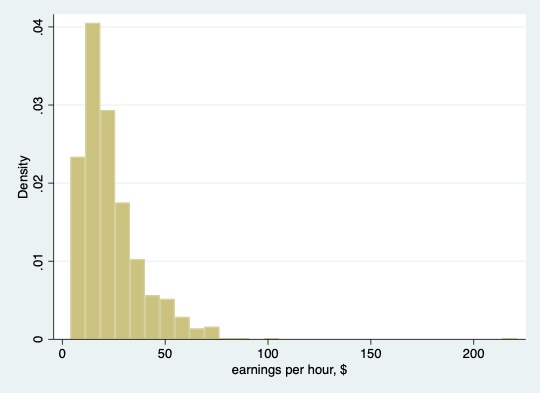
\includegraphics[scale = 0.38]{Hist_wage.jpg}
\end{center}
\end{frame}
%---------------------------------------------------------

%---------------------------------------------------------
\begin{frame}[fragile,t]
\frametitle{(a2) Summary statistics and histogram for 
EDUCATION}

\vspace{15mm}

25\% of the people had up to 12 years of education.  

\vspace{5mm}

\begin{center}
\setlength{\tabcolsep}{6pt}
\begin{tabular}{|c|c|c|c|c|c|c|c|}
\hline
variable &	$n$ & min & 25th qtile & median & mean  & 75th qtile &max \\
\hline
$educ$ & 1200 & 0 & 12.0 & 14.0 & 14.2 & 16.0 & 21.0\\
\hline
\end{tabular}
\end{center}
\hyperlink{Percentiles}{\beamerbutton{Percentiles}}
\end{frame}
%---------------------------------------------------------

%---------------------------------------------------------
\begin{frame}[fragile,t]
\frametitle{(a2) Summary statistics and histogram for 
EDUCATION}

The spike at 12 years of education describes those who finished their education at the end of high school. There are a few observations at less than 12, representing those who did not complete high school.\\

\begin{wrapfigure}{r}{0.5\textwidth}
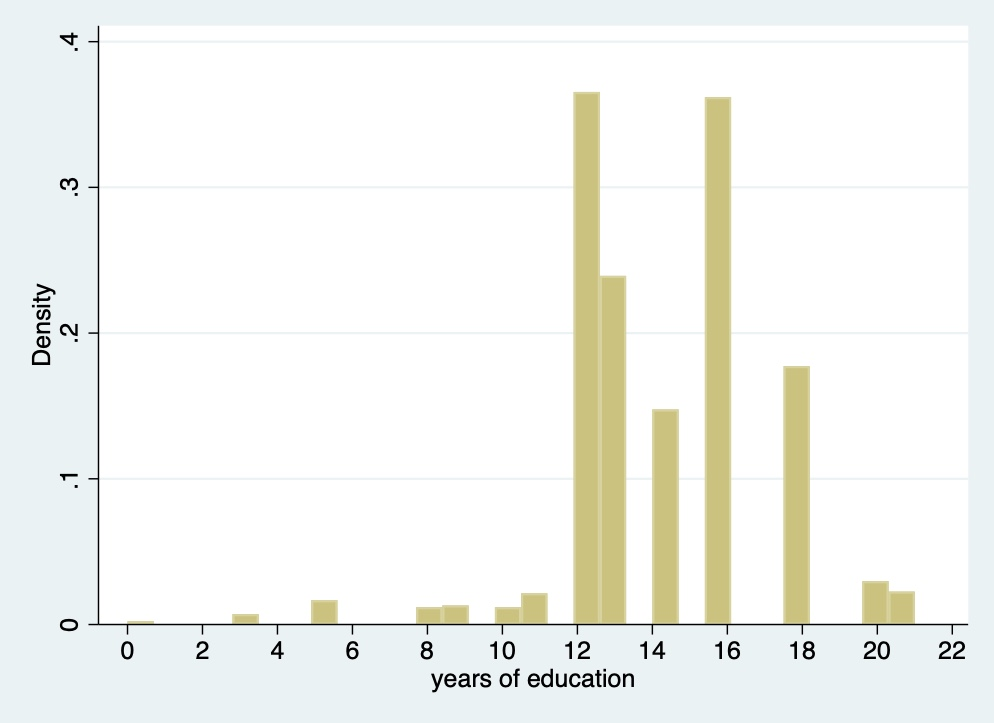
\includegraphics[scale = 0.16]{Hist_educ.jpg}
\end{wrapfigure}

\vspace{5mm}

Spikes at 13 and 14 years are people who had 1 or 2 years at college. Spike at 16 years describes those who completed a 4-year college degree, while those at 18 and 21 years represent a master's degree, and further education such as a PhD, respectively. 

\end{frame}
%---------------------------------------------------------

%---------------------------------------------------------
\begin{frame}[fragile,t]
\frametitle{(b1) Scatterplot}
\begin{center}
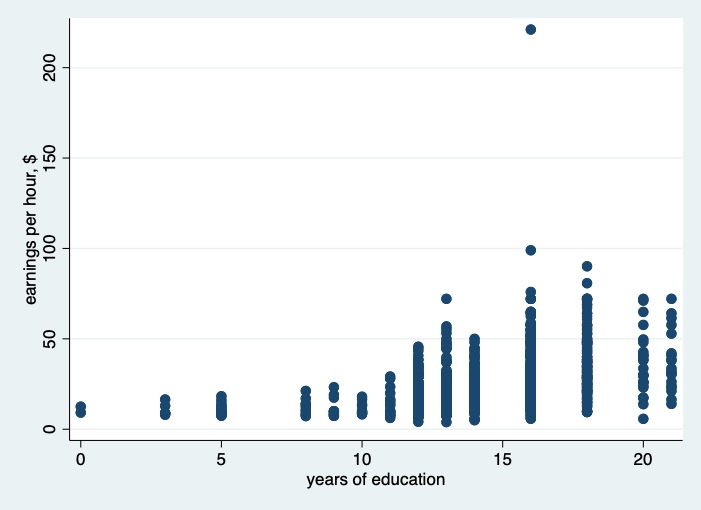
\includegraphics[width=0.7\textwidth]{scatterplot.jpg} 
\end{center}
\item There appears to be a \textit{positive} relationship between wage and education.
\hyperlink{association}{\beamerbutton{association}}
\end{frame}
%---------------------------------------------------------

%---------------------------------------------------------
\begin{frame}[fragile,t]
\frametitle{(b2) Covariance and Correlation}

\vspace{15mm}

The sample covariance and correlation also suggest a \textit{positive} relationship between wage and education.
$$\Cov(wage,educ) = 20.029 \qquad \Corr(wage,educ)=0.455$$
\hyperlink{association}{\beamerbutton{association}}
\end{frame}
%---------------------------------------------------------

%---------------------------------------------------------
\begin{frame}[fragile,t]
\frametitle{(c) Linear regression model}
\begin{center}
    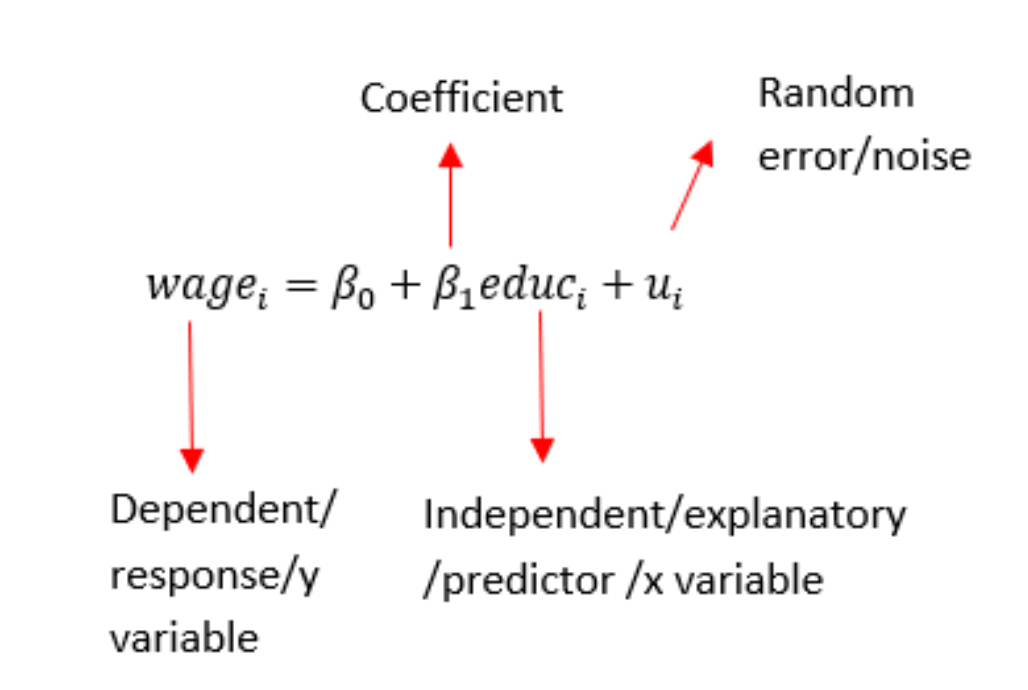
\includegraphics[scale = 0.5]{regression.png}
\end{center}
\end{frame}
%---------------------------------------------------------

%---------------------------------------------------------
\begin{frame}[fragile,t]
\frametitle{(c1) Estimation results}
$$\underset{(se)}{\widehat{wage}} = \underset{(1.9624)}{-10.4000} +  \underset{(0.1354)}{2.3968} \cdot educ \qquad R^2=0.2073 \quad SER=13.553$$ \\
%$$\widehat{wage} = -10.4000 + 2.3968 \cdot educ$$ 
%(Standard errors in parenthesis)	\\ 	
\begin{itemize}
    \item $\hat{\beta_1}:$ The slope estimate 2.3968 suggests that an extra year of education \textit{is associated with} an increase in hourly wage rate by \$2.3968 \textit{on average}.  \\
    \vspace{3mm}
    \item $\hat{\beta_0}:$  The intercept estimate -10.4 represents the estimated average hourly wage rate of a worker with no years of education. It should not be considered meaningful as it is not possible to have a negative hourly wage rate. \\
\end{itemize}
\end{frame}
%---------------------------------------------------------

%---------------------------------------------------------
\begin{frame}[fragile,t]
\frametitle{(c2) Scatterplot with regression line}
\begin{figure}
    \centering
    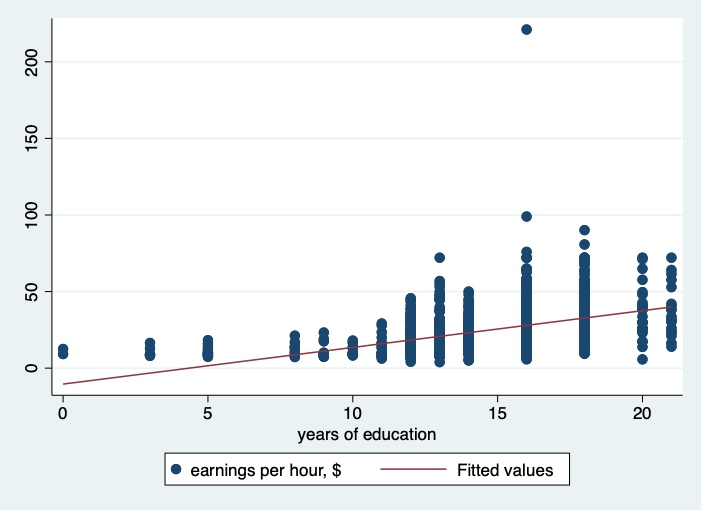
\includegraphics[scale = 0.4]{newscatterplot.jpg}
    \caption{}
    \label{fig:my_label}
\end{figure}
\end{frame}
%---------------------------------------------------------

%---------------------------------------------------------
\begin{frame}[fragile,t]
\frametitle{(d) Linear regression with new variable lnwage}\label{(d)}

\textbf{Log-Level model:}
$$
lnwage_i = \gamma_0 + \gamma_1.educ_i + \epsilon_i
$$

Estimation results:
$$\underset{(se)}{\widehat{lnwage}} = \underset{(0.070)}{1.5968} +  \underset{(0.0048)}{0.0988} \cdot educ \qquad R^2=0.2557 \quad SER= 0.4847$$ \\
\begin{itemize}
    \item $\hat{\gamma_1}$: The slope estimate 0.0988 suggests that an extra year of education \textit{is associated with} an increase in hourly wage rate by 9.88\% \textit{on average}.
    \item Brief proof:
    $$
    \Delta log(wage) = \gamma_1 \Delta educ \Longrightarrow \%\Delta wage = 100 \gamma_1 \Delta educ\\
    \hspace{10mm}\text{since } \Delta log(x) = log(x_1) - log(x_0) \approx \frac{x_1-x_0}{x_0} = \frac{\Delta x}{x} = \frac{\%\Delta x}{100}
    
    $$
\end{itemize}
\hyperlink{log-level}{\beamerbutton{log-level}}

\end{frame}
%---------------------------------------------------------

%---------------------------------------------------------
\begin{frame}[fragile,t]
\frametitle{(e) Linear regression for subgroups}
\vspace{5mm}
\begin{center}
\begin{threeparttable}
\setlength{\tabcolsep}{4pt}
\begin{tabular}{lcccc}
\hline
\multicolumn{5}{l}{Dependent variable: Log of hourly wage}\\
\hline
& (1) & (2) & (3) & (4) \\ 
\cline{2-5}
& Male & Female & White & Black \\
\hline
Years of education & \textcolor{red}{0.095} & \textcolor{red}{0.114} & \textcolor{green}{0.099} & \textcolor{green}{0.090} \\
& (0.006) & (0.008) & (0.005) & (0.017) \\
Constant & 1.724 & 1.272 & 1.603  & 1.638 \\
& (0.088) & (0.113) & (0.074) & (0.239) \\
& & & & \\
$N$ & 672 & 528 & 1095 & 105 \\
$R^2$ & 0.263 & 0.297& 0.260 & 0.210\\
$SER$ & 0.481 & 0.470 & 0.487 & 0.452 \\
\hline
%\footnotesize
%\multicolumn{5}{l}{Note: Standard errors in parenthesis}\\
\end{tabular}
\\
\begin{tablenotes}[flushleft]
\footnotesize
Note: Standard errors are in parenthesis.
\end{tablenotes}
\end{threeparttable}
\end{center}
\end{frame}
%---------------------------------------------------------

%---------------------------------------------------------
\begin{frame}[fragile,t]
\frametitle{(e) Linear regression for subgroups}
\vspace{3mm}
The percentage increase in hourly wage associated with an extra year of education:
\vspace{3mm}
\begin{itemize}
    \item is larger for female workers (11.4\% per year) than for male workers (9.5\% per year) on average.
    \item is larger for white workers (9.9\% per year) than for black workers (9\% per year) on average.
    \vspace{3mm}
\end{itemize}
\end{frame}
%---------------------------------------------------------

%---------------------------------------------------------
\begin{frame}[fragile,t]
\frametitle{(g) Least squares residuals}
\begin{center}
    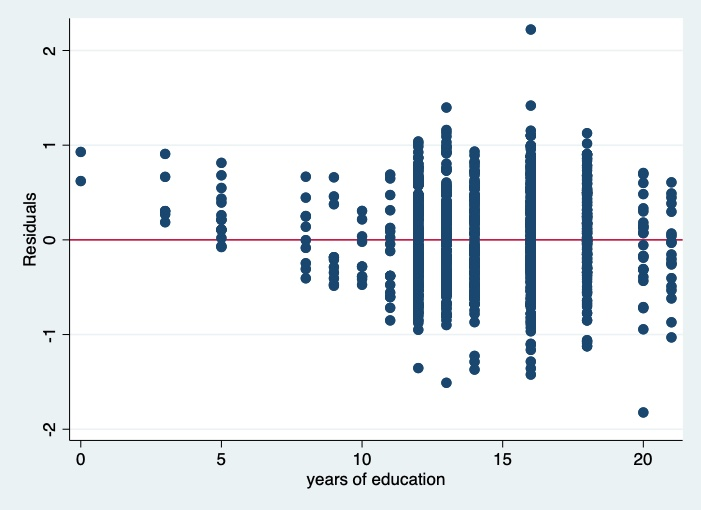
\includegraphics[scale = 0.3]{residuals.jpg}
\end{center}
\item As $educ$ increases, the spread of the residuals also increases, suggesting that the error variance is larger for larger values of $educ$ - a violation of assumption \textbf{SR.5 homoskedasticity}. 
\end{frame}
%---------------------------------------------------------

%---------------------------------------------------------
\begin{frame}[fragile,t]
\frametitle{Percentiles - Definition}\label{Percentiles}
The \textbf{$p^{th}$ percentile} is a value such that $p$ percent of the observations fall below or at that value. 

\begin{itemize}
    \item The $50^{th}$ percentile is usually referred to as the \textbf{median} ($p = 50$):
    50\% of the observations fall below or at it and 50\% above it. 
\end{itemize}
\begin{center}
    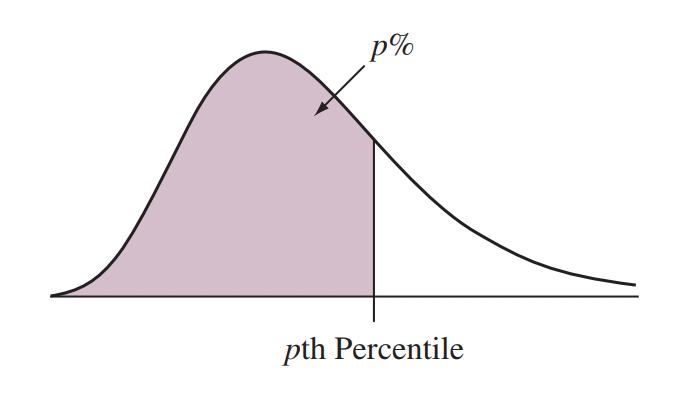
\includegraphics[scale = 0.5]{Percentiles.png}
\end{center}
\hyperlink{a1)}{\beamerbutton{(a1)}}
\end{frame}
%---------------------------------------------------------

%---------------------------------------------------------
\begin{frame}[fragile,t]
\frametitle{Percentiles - Example}

You are the fourth tallest person in a group of 15. 

\vspace{3mm}

$\Longrightarrow$ 80\% of people are shorter than or as high as you:
\begin{center}
    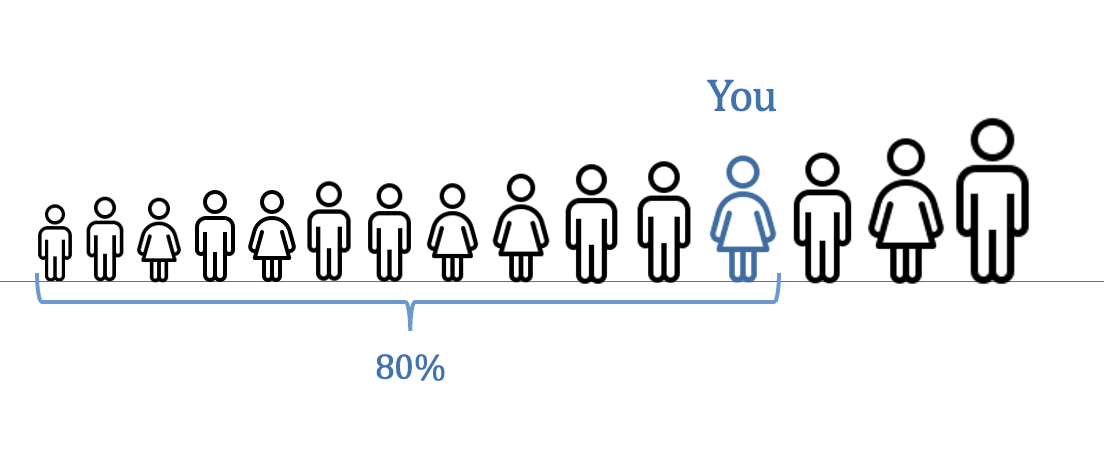
\includegraphics[scale = 0.5]{Percentiles - Example.png}
\end{center}
That means you are at the $80^{th}$ percentile.

\vspace{3mm}

If your height is 1.75m then "1.75m" is the $80^{th}$ percentile height in that group.
\hyperlink{a1)}{\beamerbutton{(a1)}}
\end{frame}
%---------------------------------------------------------

%---------------------------------------------------------
\begin{frame}[fragile,t]
\frametitle{Percentiles - Quantiles}
Three useful percentiles are the \textbf{quartiles}. The quartiles split distribution into four parts, each containing one quarter (25\%) of the observations. 

\begin{center}
    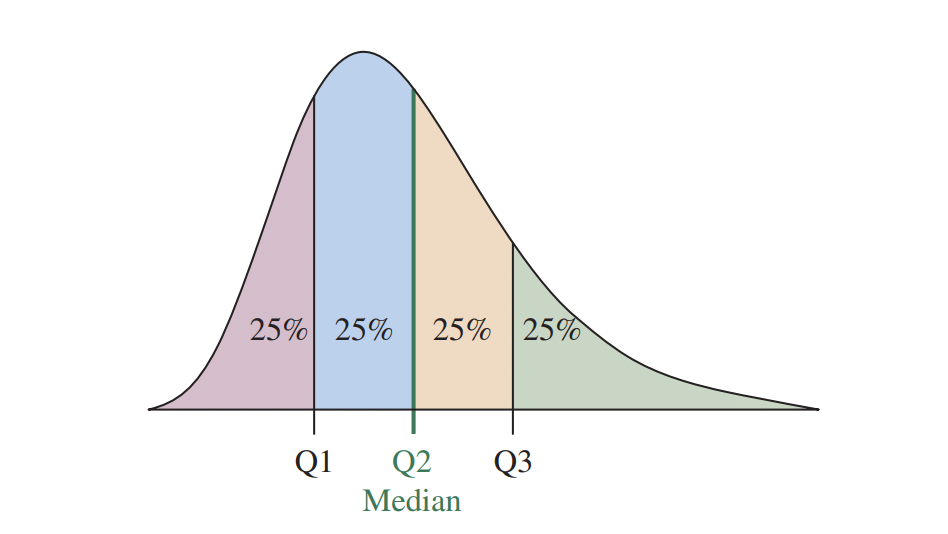
\includegraphics[scale = 0.4]{Quantiles.png}
\end{center}

\begin{itemize}
    \item The \textbf{first quartile} has $p = 25$, so it is the $25^{th}$ percentile.
    \item The \textbf{second quartile} has $p = 50$, so it is the $50^{th}$ percentile, which is the median.
    \item The \textbf{third quartile} has $p = 75$, so it is the $75^{th}$ percentile. 
\end{itemize}
\hyperlink{a1)}{\beamerbutton{(a1)}}
\end{frame}
%---------------------------------------------------------

%---------------------------------------------------------
\begin{frame}[fragile,t]
\frametitle{Skewed Distribution - Definition}
\begin{figure}
    \centering
    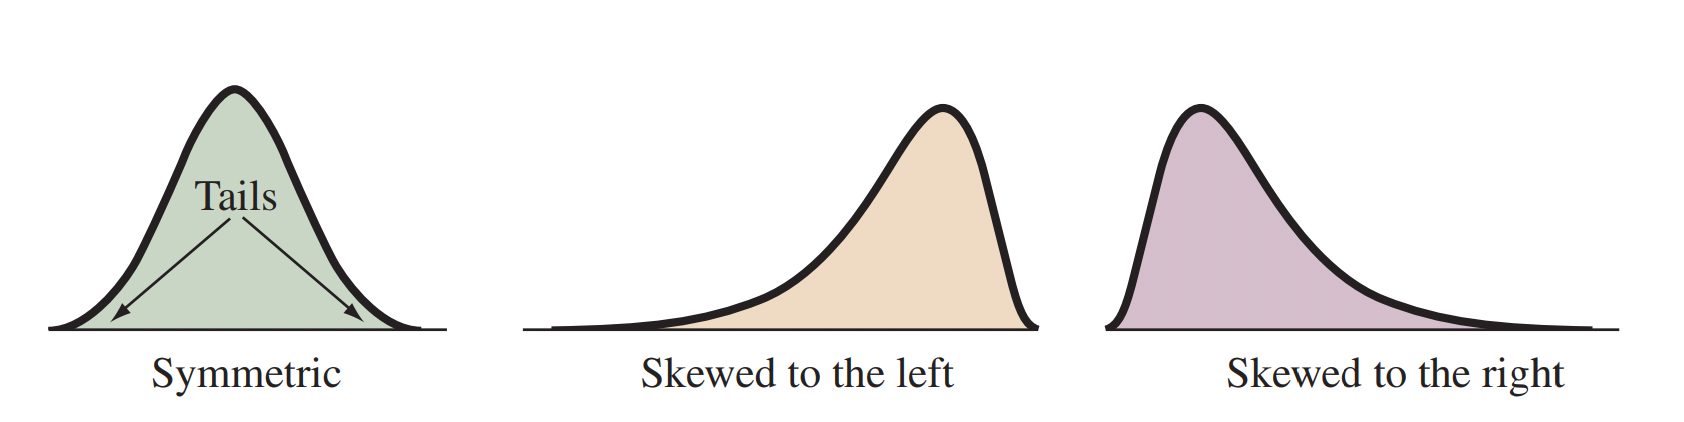
\includegraphics[scale = 0.4]{Distribution_Shape.png}
    \caption{Curves for Distributions Illustrating Symmetry and Skew}
    \label{fig:my_label}
\end{figure}

To \textbf{skew} means to stretch in one direction.
\begin{itemize}
    \item A distribution is \textit{skewed to the left} if left tail is longer than right tail.
    \item A distribution is \textit{skewed to the right} if right tail is longer than left tail.
    \item A left-skewed distribution stretches to the left and A right-skewed distribution stretches to the right.
\end{itemize}
\hyperlink{a1)}{\beamerbutton{(a1)}}
\end{frame}
%---------------------------------------------------------
%---------------------------------------------------------
\begin{frame}[fragile,t]
\frametitle{Skewed Distribution - Example}
\begin{center}
    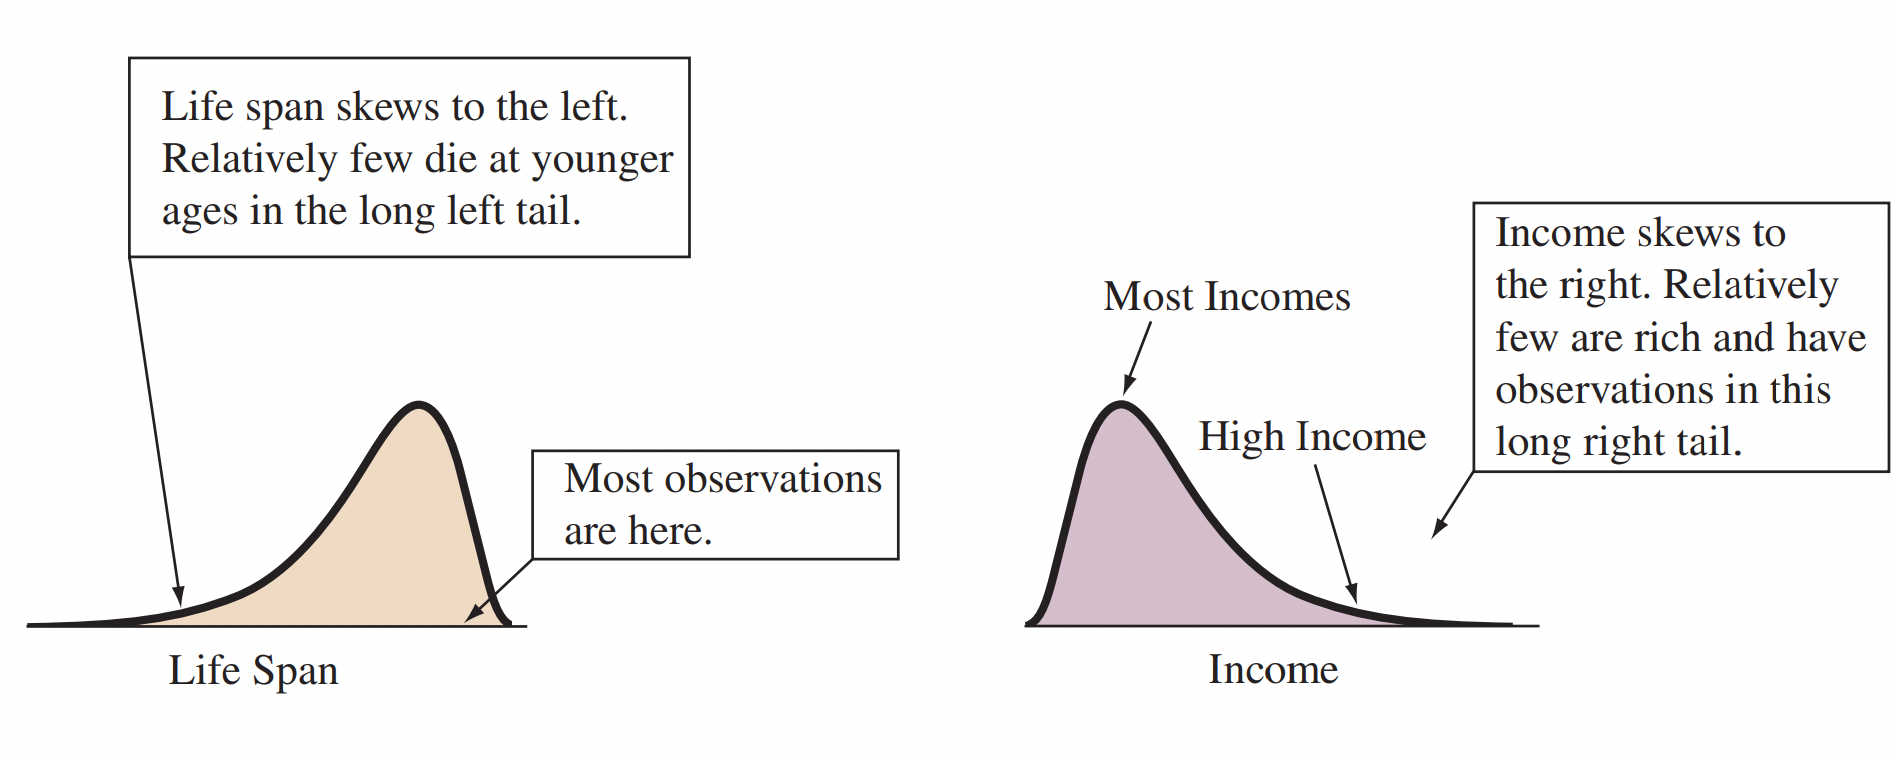
\includegraphics[scale = 0.3]{Distribution_Skew_Eg.png}
    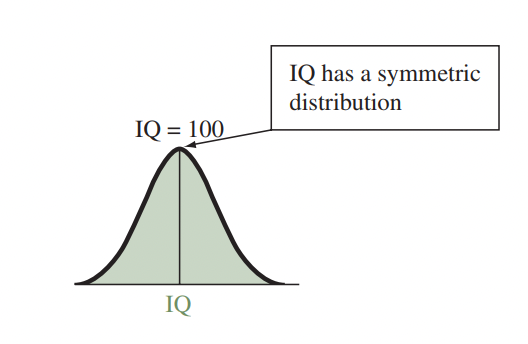
\includegraphics[scale = 0.55]{Distribution_Sym_Eg.png}
\end{center}
\hyperlink{a1)}{\beamerbutton{(a1)}}
\end{frame}
%---------------------------------------------------------

%---------------------------------------------------------
\begin{frame}[fragile,t]
\frametitle{Skewness}
Skewness measures \textbf{the degree and direction of asymmetry}.
\begin{equation*}
\text{skew[X]} =\mathrm{E}\left[\left(\frac{X-\mu}{\sigma}\right)^{3}\right]=\frac{\mu_{3}}{\sigma^{3}}
\end{equation*}
\begin{center}
    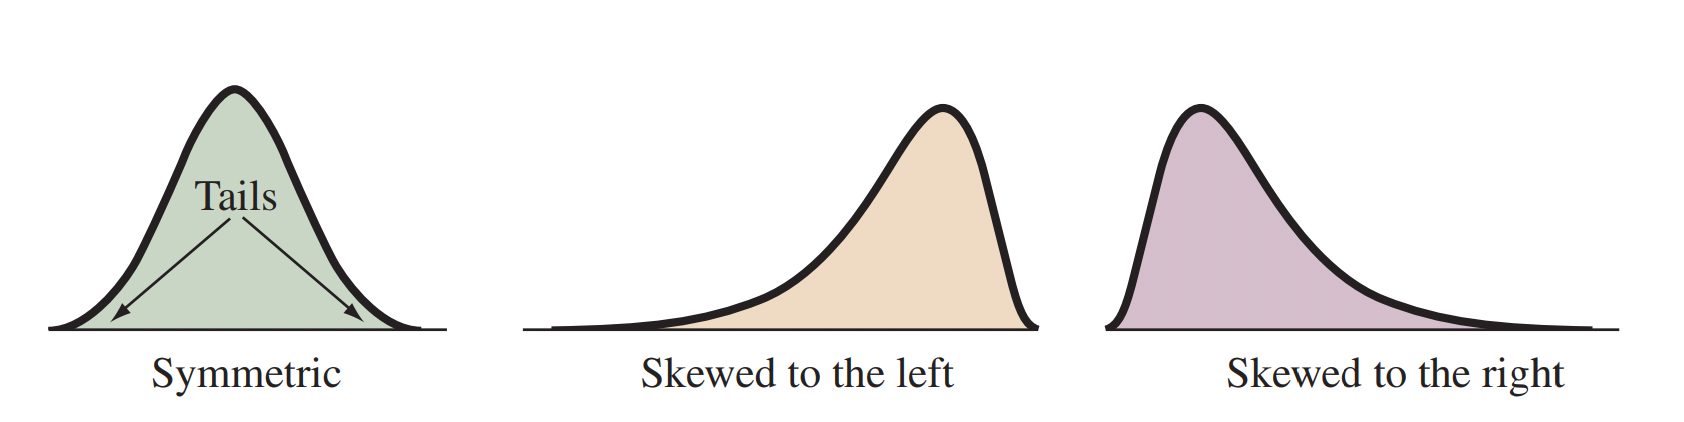
\includegraphics[scale = 0.4]{Distribution_Shape.png}
\end{center}

\begin{itemize}
    \item A \textit{symmetric} distribution has a skewness of \textit{0}. 
    \item A \textit{left-skewed} distribution has a \textit{negative} skewness.
    \item A \textit{right-skewed} distribution has a \textit{positive} skewness.
\end{itemize}
\hyperlink{a1)}{\beamerbutton{(a1)}}
\end{frame}
%---------------------------------------------------------

%---------------------------------------------------------
\begin{frame}[fragile,t]
\frametitle{Kurtosis}
\begin{center}
        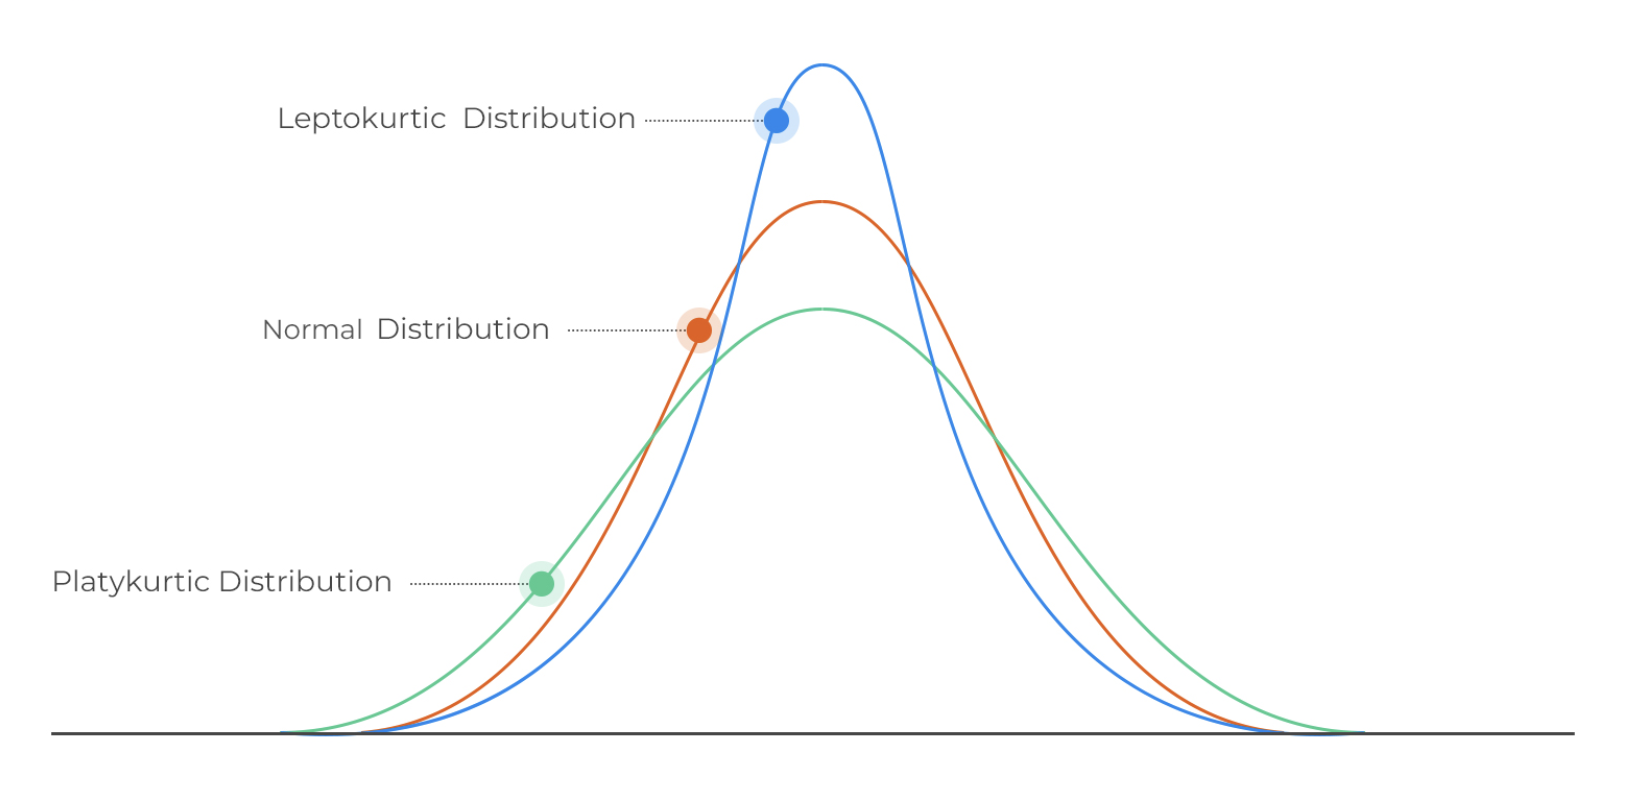
\includegraphics[scale = 0.3]{Distribution_Kurtosis.png}
\end{center}
Kurtosis is a measure of \textit{\textbf{the heaviness of the tails}} of a distribution. 
\begin{equation*}
\text{Kurt}[X]=\mathds{E}\left[\left(\frac{X-\mu}{\sigma}\right)^{4}\right]=\frac{\mu_{4}}{\sigma^{4}},
\end{equation*}
\hyperlink{a1)}{\beamerbutton{(a1)}}
\end{frame}
%---------------------------------------------------------

%---------------------------------------------------------
\begin{frame}[fragile,t]
\frametitle{Kurtosis (cont.)}
\begin{center}
        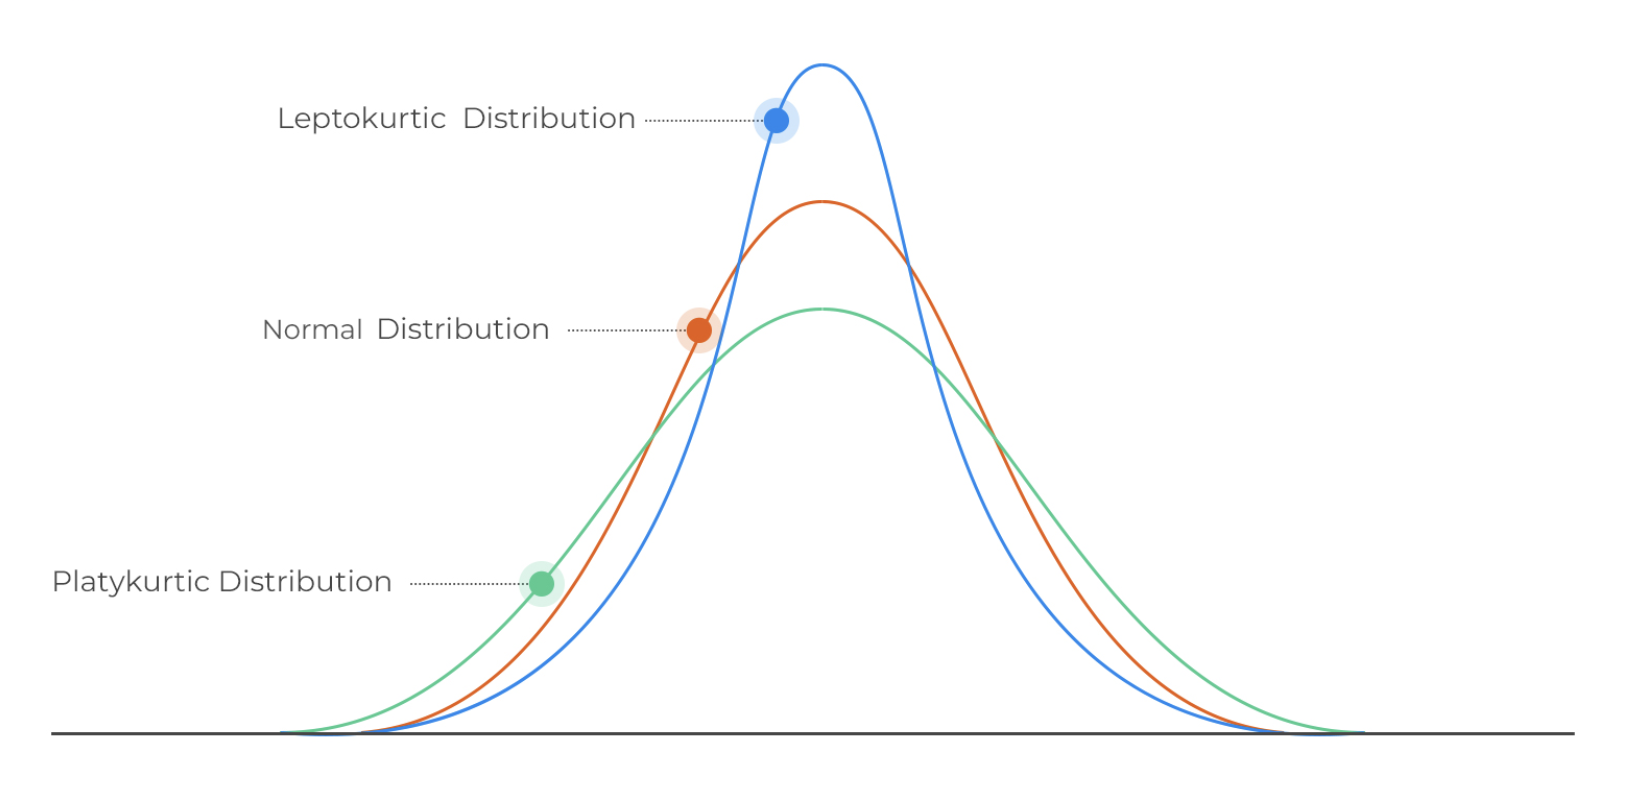
\includegraphics[scale = 0.3]{Distribution_Kurtosis.png}
\end{center}
Kurtosis is a measure of \textit{\textbf{the heaviness of the tails}} of a distribution. 
\begin{itemize}
    \item A \textcolor{red}{normal} distribution has a kurtosis of \textcolor{red}{3}.
    \item \textcolor{green}{Heavy tailed} distributions will have kurtosis \textcolor{green}{greater than 3}.
    \item \textcolor{blue}{Light tailed} distributions will have kurtosis \textcolor{blue}{less than 3}.
\end{itemize}
\hyperlink{a1)}{\beamerbutton{(a1)}}
\end{frame}
%---------------------------------------------------------

%---------------------------------------------------------
\begin{frame}[fragile,t]
\frametitle{Association - Scatterplot}\label{association}
Looking for \textbf{trend} of the \textbf{association} between two quantitative variables:
\begin{itemize}
    \item \textbf{Positive association}: As $x$ goes up, $y$ tends to go up.
    \item \textbf{Negative association}: As $x$ goes up, $y$ tends to go down.
\end{itemize}
\begin{center}
    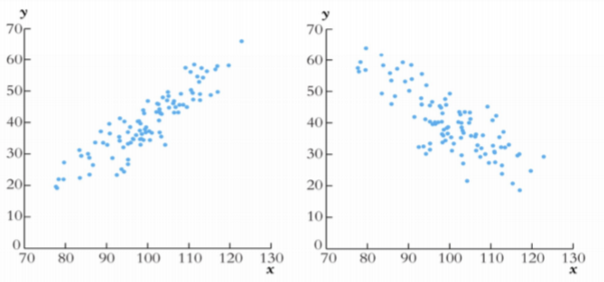
\includegraphics[]{Scatterplot.png}
\end{center}
\hyperlink{b1)}{\beamerbutton{(b1)}}
\end{frame}
%---------------------------------------------------------

%---------------------------------------------------------
\begin{frame}[fragile,t]
\frametitle{Association - Correlation}
Summarizing \textbf{direction} and \textbf{strength} of the \textbf{linear} (straight-line) \textbf{association} between two quantitative variables. 
\begin{equation}
    r==\frac{1}{n-1} \Sigma\left(\frac{x-\bar{x}}{s_{x}}\right)\left(\frac{y-\bar{y}}{s_{y}}\right)
\end{equation}
Correlation coefficient $r$ takes values between -1 and +1.
\begin{itemize}
    \item \textbf{Direction}
    \begin{itemize}
        \item $r>0$ indicates a positive association
        \item $r<0$ indicates a negative association
    \end{itemize}
    \item \textbf{Strength}
    \begin{itemize}
        \item The closer $r$ is to +/-1 the closer the data points fall to a straight line, and the stronger the linear association is.
        \item The closer $r$ is to 0, the weaker the linear association is.
    \end{itemize} 
\end{itemize}
\hyperlink{b2)}{\beamerbutton{(b2)}}
\end{frame}
%---------------------------------------------------------

%---------------------------------------------------------
\begin{frame}[fragile,t]
\frametitle{Association - Correlation (cont.)}
\begin{center}
    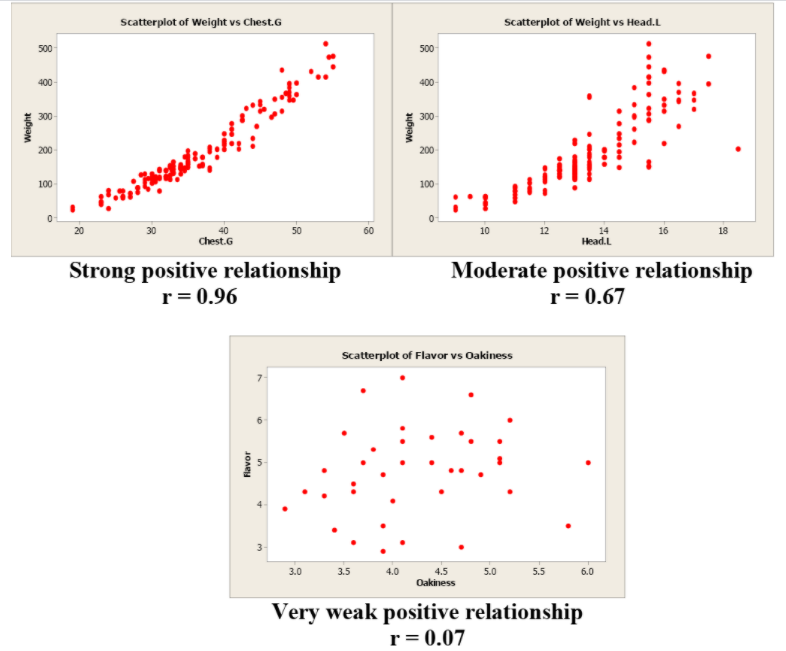
\includegraphics[scale = 0.6]{Positive_Correlation.png}
\end{center}
\end{frame}
%---------------------------------------------------------

%---------------------------------------------------------
\begin{frame}[fragile,t]
\frametitle{Association - Correlation (cont.)}
\begin{center}
    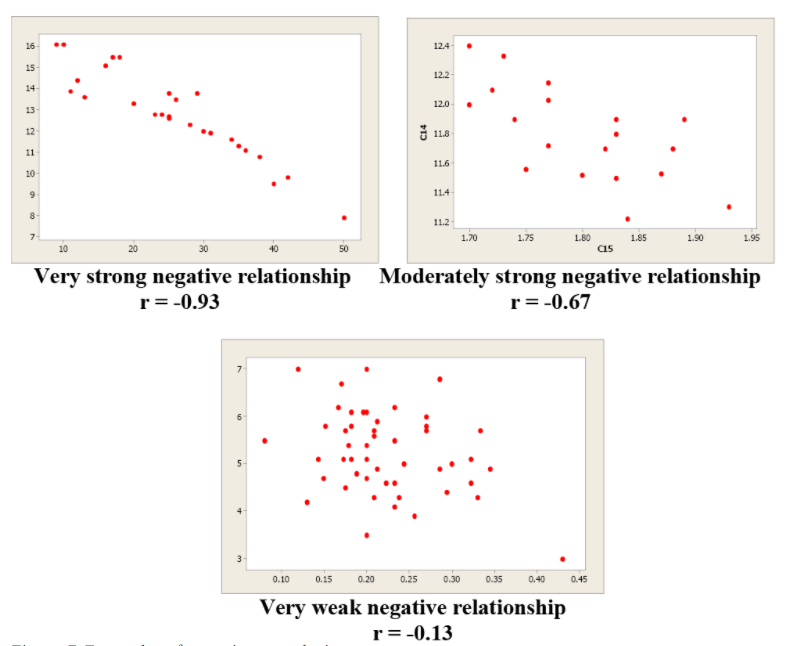
\includegraphics[scale = 0.6]{Negative_Correlation.png}
\end{center}
\end{frame}
%---------------------------------------------------------

%---------------------------------------------------------
\begin{frame}[fragile,t]
\frametitle{Association - Correlation (cont.)}
\textcolor{red}{(!)} Correlation \textcolor{red}{poorly describes} the association when the relationship is \textcolor{red}{curved (non-linear)}. 
\begin{center}
    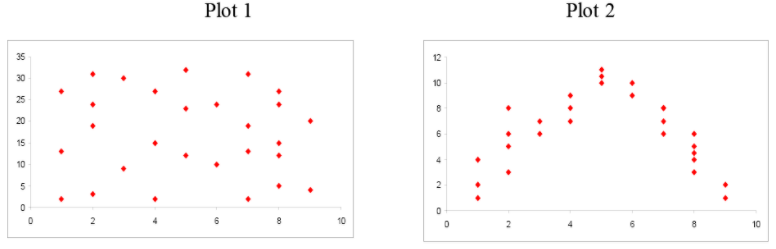
\includegraphics[scale = 0.8]{Caution_Correlation.png}
\end{center}
For this U-shaped relationship, the correlation is 0 (or close to 0), even though the variables are strongly associated. Ignoring the scatterplot could result in a serious mistake when describing the relationship between two variables.
\end{frame}
%---------------------------------------------------------

%---------------------------------------------------------
\begin{frame}[fragile,t]
\frametitle{Association - In Practice}
\begin{enumerate}
    \item When you investigate the relationship between two quantitative variables, always \textbf{begin with a scatterplot}. This graph allows you to look for patterns (both linear and non-linear). 
    \vspace{3mm}
    \item The next step is to quantitatively describe the strength and direction of the linear relationship (an approximate straight-line relationship) using  the \textbf{correlation coefficient “r”}. 
    \vspace{3mm}
    \item Once you have established that a linear relationship exists, you can take the next step in model building.
\end{enumerate}
\end{frame}
%---------------------------------------------------------

%---------------------------------------------------------
\begin{frame}[fragile,t]
\frametitle{Functional Forms Involving Logarithms}\label{log-level}
Constant unit change/ Constant percentage change/ Constant elasticity?
\begin{center}
    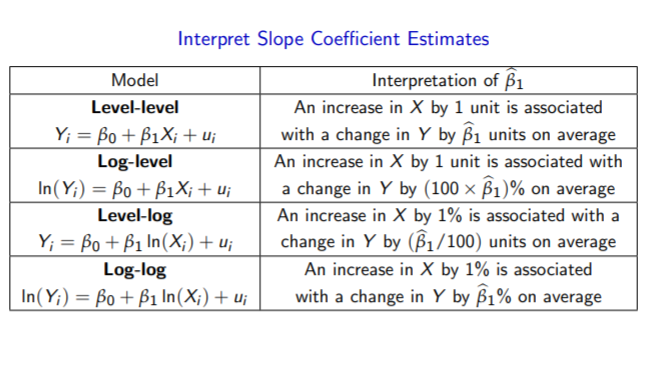
\includegraphics[scale = 0.9]{Regression_with_Log.png}
\end{center}
\end{frame}
%---------------------------------------------------------

%---------------------------------------------------------
\begin{frame}[fragile,t]
\frametitle{Functional Forms Involving Logarithms (cont.)}
Why \textbf{logarithmic transformation}?
\vspace{3mm}
\begin{itemize}
    \item Meaningful interpretation: reasonable, consistent with economic theories.
    \vspace{3mm}
    \item Yields a distribution that is closer to normal $\Longrightarrow$ better for inference purpose.
\end{itemize}
\hyperlink{d)}{\beamerbutton{(d)}}
\end{frame}
%---------------------------------------------------------

%---------------------------------------------------------
\end{document}